\documentclass[conference]{IEEEtran}
% \special{papersize=8.5in,11in}

\title{Development of Motion Planning Algorithms for Inchworm Robots\\
    {\footnotesize A WPI RBE 550 Project Spring 2021}
}

\author{
    \IEEEauthorblockN{Alex Tacescu}
    \IEEEauthorblockA{\textit{Robotics Engineering} \\
    \textit{Worcester Polytechnic Institute}\\
    Worceser, Massachusetts \\
    actacescu@wpi.edu}
\and
    \IEEEauthorblockN{Nicole Kuberka}
    \IEEEauthorblockA{\textit{Robotics Engineering} \\
    \textit{Worcester Polytechnic Institute}\\
    Worceser, Massachusetts \\
    nlkuberka@wpi.edu}
\and
    \IEEEauthorblockN{Meha Mohapatra}
    \IEEEauthorblockA{\textit{Robotics Engineering} \\
    \textit{Worcester Polytechnic Institute}\\
    Worceser, Massachusetts \\
    mmohapatra@wpi.edu}
\and
    \IEEEauthorblockN{Sri Kalimani}
    \IEEEauthorblockA{\textit{Robotics Engineering} \\
    \textit{Worcester Polytechnic Institute}\\
    Worceser, Massachusetts \\
    skalimani@wpi.edu}
}

% Import setup file with includes
% Some very useful LaTeX packages include:
% (uncomment the ones you want to load)

%%%%%%%%%%%%%%%%%%%%%%%%%%%%%%%%%%%%%
% ***** Misc Utility Packages ***** %
%%%%%%%%%%%%%%%%%%%%%%%%%%%%%%%%%%%%%

%\usepackage{ifpdf}
% Heiko Oberdiek's ifpdf.sty is very useful if you need conditional
% compilation based on whether the output is pdf or dvi.
% usage:
% \ifpdf
%   % pdf code
% \else
%   % dvi code
% \fi
% The latest version of ifpdf.sty can be obtained from:
% http://www.ctan.org/pkg/ifpdf
% Also, note that IEEEtran.cls V1.7 and later provides a builtin
% \ifCLASSINFOpdf conditional that works the same way.
% When switching from latex to pdflatex and vice-versa, the compiler may
% have to be run twice to clear warning/error messages.

%%%%%%%%%%%%%%%%%%%%%%%%%%%%%%%%%
% ***** Citation Packages ***** %
%%%%%%%%%%%%%%%%%%%%%%%%%%%%%%%%%

\usepackage[
    style=ieee,
    backend=biber,
    sortcites=true,
    sorting=nyt,
%    isbn=false,
   url=true,
   doi=true,
%    eprint=false,
    hyperref=false,
    backref=false,
%    firstinits=false,
    bibencoding=utf8
]{biblatex}
\usepackage{csquotes}

% \usepackage{cite}
% cite.sty was written by Donald Arseneau
% V1.6 and later of IEEEtran pre-defines the format of the cite.sty package
% \cite{} output to follow that of the IEEE. Loading the cite package will
% result in citation numbers being automatically sorted and properly
% "compressed/ranged". e.g., [1], [9], [2], [7], [5], [6] without using
% cite.sty will become [1], [2], [5]--[7], [9] using cite.sty. cite.sty's
% \cite will automatically add leading space, if needed. Use cite.sty's
% noadjust option (cite.sty V3.8 and later) if you want to turn this off
% such as if a citation ever needs to be enclosed in parenthesis.
% cite.sty is already installed on most LaTeX systems. Be sure and use
% version 5.0 (2009-03-20) and later if using hyperref.sty.
% The latest version can be obtained at:
% http://www.ctan.org/pkg/cite
% The documentation is contained in the cite.sty file itself.

% \def\BibTeX{{\rm B\kern-.05em{\sc i\kern-.025em b}\kern-.08em
%     T\kern-.1667em\lower.7ex\hbox{E}\kern-.125emX}}

%%%%%%%%%%%%%%%%%%%%%%%%%%%%%%%%%
% ***** Graphics Packages ***** %
%%%%%%%%%%%%%%%%%%%%%%%%%%%%%%%%%

\usepackage{graphicx}
\usepackage{hyperref}
% graphicx was written by David Carlisle and Sebastian Rahtz. It is
% required if you want graphics, photos, etc. graphicx.sty is already
% installed on most LaTeX systems. The latest version and documentation
% can be obtained at: 
% http://www.ctan.org/pkg/graphicx
% Another good source of documentation is "Using Imported Graphics in
% LaTeX2e" by Keith Reckdahl which can be found at:
% http://www.ctan.org/pkg/epslatex
%
% latex, and pdflatex in dvi mode, support graphics in encapsulated
% postscript (.eps) format. pdflatex in pdf mode supports graphics
% in .pdf, .jpeg, .png and .mps (metapost) formats. Users should ensure
% that all non-photo figures use a vector format (.eps, .pdf, .mps) and
% not a bitmapped formats (.jpeg, .png). The IEEE frowns on bitmapped formats
% which can result in "jaggedy"/blurry rendering of lines and letters as
% well as large increases in file sizes.
%
% You can find documentation about the pdfTeX application at:
% http://www.tug.org/applications/pdftex

%%%%%%%%%%%%%%%%%%%%%%%%%%%%%
% ***** Math Packages ***** %
%%%%%%%%%%%%%%%%%%%%%%%%%%%%%

\usepackage{amsmath}
\usepackage{amssymb}
\usepackage{amsfonts}
% A popular package from the American Mathematical Society that provides
% many useful and powerful commands for dealing with mathematics.
%
% Note that the amsmath package sets \interdisplaylinepenalty to 10000
% thus preventing page breaks from occurring within multiline equations. Use:
%\interdisplaylinepenalty=2500
% after loading amsmath to restore such page breaks as IEEEtran.cls normally
% does. amsmath.sty is already installed on most LaTeX systems. The latest
% version and documentation can be obtained at:
% http://www.ctan.org/pkg/amsmath

%%%%%%%%%%%%%%%%%%%%%%%%%%%%%%%%%%%%%%%%%
% ***** Specialized List Packages ***** %
%%%%%%%%%%%%%%%%%%%%%%%%%%%%%%%%%%%%%%%%%

\usepackage{algorithmic}
% algorithmic.sty was written by Peter Williams and Rogerio Brito.
% This package provides an algorithmic environment fo describing algorithms.
% You can use the algorithmic environment in-text or within a figure
% environment to provide for a floating algorithm. Do NOT use the algorithm
% floating environment provided by algorithm.sty (by the same authors) or
% algorithm2e.sty (by Christophe Fiorio) as the IEEE does not use dedicated
% algorithm float types and packages that provide these will not provide
% correct IEEE style captions. The latest version and documentation of
% algorithmic.sty can be obtained at:
% http://www.ctan.org/pkg/algorithms
% Also of interest may be the (relatively newer and more customizable)
% algorithmicx.sty package by Szasz Janos:
% http://www.ctan.org/pkg/algorithmicx

%%%%%%%%%%%%%%%%%%%%%%%%%%%%%%%%%%
% ***** Alignment Packages ***** %
%%%%%%%%%%%%%%%%%%%%%%%%%%%%%%%%%%

%\usepackage{array}
% Frank Mittelbach's and David Carlisle's array.sty patches and improves
% the standard LaTeX2e array and tabular environments to provide better
% appearance and additional user controls. As the default LaTeX2e table
% generation code is lacking to the point of almost being broken with
% respect to the quality of the end results, all users are strongly
% advised to use an enhanced (at the very least that provided by array.sty)
% set of table tools. array.sty is already installed on most systems. The
% latest version and documentation can be obtained at:
% http://www.ctan.org/pkg/array


% IEEEtran contains the IEEEeqnarray family of commands that can be used to
% generate multiline equations as well as matrices, tables, etc., of high
% quality.

%%%%%%%%%%%%%%%%%%%%%%%%%%%%%%%%%%
% ***** Subfigure Packages ***** %
%%%%%%%%%%%%%%%%%%%%%%%%%%%%%%%%%%

%\ifCLASSOPTIONcompsoc
%  \usepackage[caption=false,font=normalsize,labelfont=sf,textfont=sf]{subfig}
%\else
%  \usepackage[caption=false,font=footnotesize]{subfig}
%\fi
% subfig.sty, written by Steven Douglas Cochran, is the modern replacement
% for subfigure.sty, the latter of which is no longer maintained and is
% incompatible with some LaTeX packages including fixltx2e. However,
% subfig.sty requires and automatically loads Axel Sommerfeldt's caption.sty
% which will override IEEEtran.cls' handling of captions and this will result
% in non-IEEE style figure/table captions. To prevent this problem, be sure
% and invoke subfig.sty's "caption=false" package option (available since
% subfig.sty version 1.3, 2005/06/28) as this is will preserve IEEEtran.cls
% handling of captions.
% Note that the Computer Society format requires a larger sans serif font
% than the serif footnote size font used in traditional IEEE formatting
% and thus the need to invoke different subfig.sty package options depending
% on whether compsoc mode has been enabled.
%
% The latest version and documentation of subfig.sty can be obtained at:
% http://www.ctan.org/pkg/subfig

%%%%%%%%%%%%%%%%%%%%%%%%%%%%%%
% ***** Float Packages ***** %
%%%%%%%%%%%%%%%%%%%%%%%%%%%%%%

%\usepackage{fixltx2e}
% fixltx2e, the successor to the earlier fix2col.sty, was written by
% Frank Mittelbach and David Carlisle. This package corrects a few problems
% in the LaTeX2e kernel, the most notable of which is that in current
% LaTeX2e releases, the ordering of single and double column floats is not
% guaranteed to be preserved. Thus, an unpatched LaTeX2e can allow a
% single column figure to be placed prior to an earlier double column
% figure.
% Be aware that LaTeX2e kernels dated 2015 and later have fixltx2e.sty's
% corrections already built into the system in which case a warning will
% be issued if an attempt is made to load fixltx2e.sty as it is no longer
% needed.
% The latest version and documentation can be found at:
% http://www.ctan.org/pkg/fixltx2e


%\usepackage{stfloats}
% stfloats.sty was written by Sigitas Tolusis. This package gives LaTeX2e
% the ability to do double column floats at the bottom of the page as well
% as the top. (e.g., "\begin{figure*}[!b]" is not normally possible in
% LaTeX2e). It also provides a command:
%\fnbelowfloat
% to enable the placement of footnotes below bottom floats (the standard
% LaTeX2e kernel puts them above bottom floats). This is an invasive package
% which rewrites many portions of the LaTeX2e float routines. It may not work
% with other packages that modify the LaTeX2e float routines. The latest
% version and documentation can be obtained at:
% http://www.ctan.org/pkg/stfloats
% Do not use the stfloats baselinefloat ability as the IEEE does not allow
% \baselineskip to stretch. Authors submitting work to the IEEE should note
% that the IEEE rarely uses double column equations and that authors should try
% to avoid such use. Do not be tempted to use the cuted.sty or midfloat.sty
% packages (also by Sigitas Tolusis) as the IEEE does not format its papers in
% such ways.
% Do not attempt to use stfloats with fixltx2e as they are incompatible.
% Instead, use Morten Hogholm'a dblfloatfix which combines the features
% of both fixltx2e and stfloats:
%
% \usepackage{dblfloatfix}
% The latest version can be found at:
% http://www.ctan.org/pkg/dblfloatfix




%\ifCLASSOPTIONcaptionsoff
%  \usepackage[nomarkers]{endfloat}
% \let\MYoriglatexcaption\caption
% \renewcommand{\caption}[2][\relax]{\MYoriglatexcaption[#2]{#2}}
%\fi
% endfloat.sty was written by James Darrell McCauley, Jeff Goldberg and 
% Axel Sommerfeldt. This package may be useful when used in conjunction with 
% IEEEtran.cls'  captionsoff option. Some IEEE journals/societies require that
% submissions have lists of figures/tables at the end of the paper and that
% figures/tables without any captions are placed on a page by themselves at
% the end of the document. If needed, the draftcls IEEEtran class option or
% \CLASSINPUTbaselinestretch interface can be used to increase the line
% spacing as well. Be sure and use the nomarkers option of endfloat to
% prevent endfloat from "marking" where the figures would have been placed
% in the text. The two hack lines of code above are a slight modification of
% that suggested by in the endfloat docs (section 8.4.1) to ensure that
% the full captions always appear in the list of figures/tables - even if
% the user used the short optional argument of \caption[]{}.
% IEEE papers do not typically make use of \caption[]'s optional argument,
% so this should not be an issue. A similar trick can be used to disable
% captions of packages such as subfig.sty th\def\BibTeX{{\rm B\kern-.05em{\sc i\kern-.025em b}\kern-.08em
    % T\kern-.1667em\lower.7ex\hbox{E}\kern-.125emX}}
% For subfig.sty:
% \let\MYorigsubfloat\subfloat
% \renewcommand{\subfloat}[2][\relax]{\MYorigsubfloat[]{#2}}
% However, the above trick will not work if both optional arguments of
% the \subfloat command are used. Furthermore, there needs to be a
% description of each subfigure *somewhere* and endfloat does not add
% subfigure captions to its list of figures. Thus, the best approach is to
% avoid the use of subfigure captions (many IEEE journals avoid them anyway)
% and instead reference/explain all the subfigures within the main caption.
% The latest version of endfloat.sty and its documentation can obtained at:
% http://www.ctan.org/pkg/endfloat
%
% The IEEEtran \ifCLASSOPTIONcaptionsoff conditional can also be used
% later in the document, say, to conditionally put the References on a 
% page by themselves.

%%%%%%%%%%%%%%%%%%%%%%%%%%%%%%%%%%%%%%%%%%%%%%%
% ***** PDF, URL AND HYPERLINK PACKAGES ***** %
%%%%%%%%%%%%%%%%%%%%%%%%%%%%%%%%%%%%%%%%%%%%%%%

%\usepackage{url}
% url.sty was written by Donald Arseneau. It provides better support for
% handling and breaking URLs. url.sty is already installed on most LaTeX
% systems. The latest version and documentation can be obtained at:
% http://www.ctan.org/pkg/url
% Basically, \url{my_url_here}.




% *** Do not adjust lengths that control margins, column widths, etc. ***
% *** Do not use packages that alter fonts (such as pslatex).         ***
% There should be no need to do such things with IEEEtran.cls V1.6 and later.
% (Unless specifically asked to do so by the journal or conference you plan
% to submit to, of course. )


% correct bad hyphenation here
\hyphenation{op-tical net-works semi-conduc-tor}

%%%%%%%%%%%%%%%%%%%%%%%%%%%%%%%%%%%
% ---- Paper Specific Setup ----- %
%%%%%%%%%%%%%%%%%%%%%%%%%%%%%%%%%%%

\bibliography{ref}

\begin{document}

    % make the title area
    \maketitle

    % Add abstract
    \begin{abstract}
    This document is a model and instructions for \LaTeX.
    This and the IEEEtran.cls file define the components of your paper [title, text, heads, etc.]. *CRITICAL: Do Not Use Symbols, Special Characters, Footnotes, 
    or Math in Paper Title or Abstract.
\end{abstract}

    % Introduction
    \section{Introduction}

We will plan the motion of a 5 DOF inchworm robot from a start to end node. As we progress in the project we plan on making the creation of the path more complex by either introducing more obstacles or adding more robots to the system. If we have time we will attempt to ferry blocks from one location to another. 

\begin{figure}[ht]
    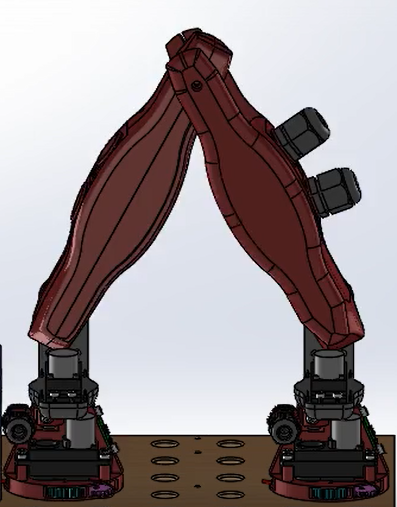
\includegraphics[width=\linewidth]{figures/InchwormPic.PNG}
    \caption{SolidWorks model of the inchworm robot used in this project \cite{PastMQP}}
    \label{fig:Inchworm}
\end{figure} 

    % Related Work
    \section{Related Work}

    % Goals
    \section{Goals}
We have created minimum, expected, and reach goals for our project. Our minimum goal is creating a fully setup simulation playground which includes a robot able to follow the gait. This simulation is necessary to test and complete the path and motion planning for our project. We will be able to visualize what the algorithm is doing and debug. The expected goals are creating a path for the robot and footstep planning for just the robot. We hope to be able to visualize the path created and see the robot taking the path by the end of our project. The reach goals we have thought about are moving with a block, creating a 3D walking gait, 3D path planning of going up walls, and implementing multiple robots into the system. Since these robots are building structures in the larger MQP our next step once we have finished our expected goals we would be moving with blocks which leads to the building of structures. The 3D walking gait would be next and have to take into account going up walls and moving around the corners of the blocks. If this gait is completed a 3D path planning algorithm could be attempted meaning adding much more complexity and destinations that could be up multiple levels of blocks. A different route we could take is adding multiple robots to the system. This would create a swarm situation where we have to account for collision detection with all robots.

\textbf{Minimum Deliverables}
\begin{itemize}
    \item Fully setup simulation playground
    \item Inchworm robot able follow the gait
\end{itemize}

\textbf{Expected Deliverables}
\begin{itemize}
    \item Functional Path planning algorithm visualized in the simulation
    \item Foot step planning for inchworm robot
    \item Inchworm robot followed layout plan in simulation
\end{itemize}

\textbf{Reach Deliverables}
\begin{itemize}
    \item Motion planning of robot with block
    \item Creation of a 3D walking gait 
    \item 3D path planning 
    \item Creating a multi-robot system
\end{itemize}


    % Proposed Methods
    \section{Proposed Methods}
In order to complete the goals we have outlined, we have split the project into a few major sections. First and foremost is the simulation environments, which will help us debug and develop our algorithms. Second major goal is to plan the path of an inchworm from one place to another, a path planning algorithm will be developed and implemented. Finally,  a motion planning algorithm will be given the path created and simulate the robot walking the path.

\subsection{Simulation Environment}
Since the Covid-19 pandemic is preventing testing with physical hardware, a full physics simulator will be used to test the motion planning software that is designed and implemented. Simple simulators will also be developed to aid in the development of complicated path planning algorithms.

RVIZ will be the tool of choice to display and loosely simulate the path planning algorithms developed. Since physics is not considered, many of the variables that are not necessary for initial development of the path planning and footstep algorithms can be isolated and temporarily removed to simplify the software. These sudo-simulators can also be turned into visualizers to better understand what the system is doing when all of the algorithms are implemented and running together.

To test the robot in a virtual playground, a Gazebo simulator will be used with a playground and inchworm model. Since Gazebo is a full physics simulator, the inchworm model will need to include mass, inertia, and a semi-accurate model of the end effector. This includes a method to approximate the magnetic end effector of the inchworm. A Gazebo Vacuum Gripper Plugin will be used to achieve this [ref both sim stuff], since the desired effect of a magnetic gripper is similar to a vacuum gripper, and developing a new plugin for Gazebo is out of the scope of this project. If we reach our expected goals, a model of the cube will be developed, which will include its own controller to simulate the connection between different cubes.

\subsection{Path Planning}
A path planning algorithm will be implemented to generate a path between the current position of the robot and the goal node, as determined by a higher-level system. The system should consider several robot conditions, including (but not limited to) inchworm step limitations, movement constraints, and collision avoidance (if the project progresses to a point where the inchworm is being tested in a cluttered environment). Several path planning algorithms are currently being considered, including A*, RTT*, and RAGS (Risk Averse Graph Section). A relatively simple algorithm (A* or RTT*) will likely be implemented first, since initially the inchworm will be tested on a perfectly level and empty playground. If time allows, RAGS [insert RAGS ref] may be implemented and compared to other algorithms, especially if the project leads to more advanced 3D graphs and maps.

The map is very important to a successful path planning algorithm. This project will initially use a simple 2 dimensional map (stored as a graph) to simplify the initial implementation of the path planning algorithm developed. If the climbing reach goal [insert ref to goal] is attempted, the map will need to consider a 3 dimensional environment. The first solution to be tested will be a “2.5” dimensional map, where the height will be added as a 3rd parameter. This may work for situations where the inchworm will only use the upward-facing face of the blocks in a structure. For situations where more advanced climbing is required, a fully 3-dimensional map will be required.

A map also needs to be generated given a playground. Perception is beyond the scope of this project, so the map will be generated based on a list of building blocks and their positions maintained by Gazebo. Initially for the 2 dimensional map, occupancy grids will be used as the map data structure, and blocks will be considered obstacles to be avoided by the robot. If the project leads to a 3 dimensional map, octrees are planned to be used as the map’s underlying data structure. One limitation that may cause issues during development is definition of what is graspable and what is not. To solve this, the occupancy grid may also contain information on the graspability of the position. This information will then be relayed back to the main path planner to be considered as a heuristic.

\subsection{Motion Planning}
The second major part of this project is the motion planning of the inchworm itself. While the path planning algorithm is in charge of determining an achievable path for the inchworm, the motion planning algorithms implemented will be in charge of actually executing that path. This major task can further be split into three major sections: inchworm kinematics, movement gaits, and footstep planning.

The 5 degree-of-freedom inchworm kinematics will be kept relatively simple, and dynamics will be automatically considered by a smart joint controller built into ROS and Gazebo. This is meant to simplify the development of the project, since dynamics of the robot is beyond the scope of this project. The overall kinematics of the inchworm will be similar to a robot arm, since the robot will have a stationary base during the movement gaits. However, two different kinematic controllers will need to be developed, depending what side of the inchworm is grounded.

The movement gaits include the general walking gait and the climbing gait. Ideally, both gaits will be combined into one main gait which can climb and walk around a playground. The gait itself will essentially be a large state machine[ref long paper]. Initially, the robot is assumed to be in a position where both end effectors are locked into the playground. The leading foot will then be unlocked and moved to the next footstep position (as generated by the footstep planner). Then the leading foot will be placed in the correct position and locked down. Finally the back foot will unlock and move to its designated footstep position, and lock down. The cycle will loop back to the beginning until the inchworm reaches its final footstep position. [ref inchworm footstep paper (if we can find it]


    % Metrics for Success
    \section{Metrics for Evaluation of Success}

    % Schedule
    \section{Schedule}
The project has been split into three different sections: development environment setup, motion planning of the inchworm robot, and path planning of the inchworm. The development environment setup effort will be spearheaded by all 4 team members. After the environment is set up, two developers will be tasked with motion planning, while the other two will develop the path planning algorithms required. If all expected deliverables are completed, the team will re-evaluate the task division for reach goals. It is important to note that 2 weeks is dedicated to schedule leeway to deal with unexpected delays and/or development problems with previous tasks.

\begin{figure}[ht]
    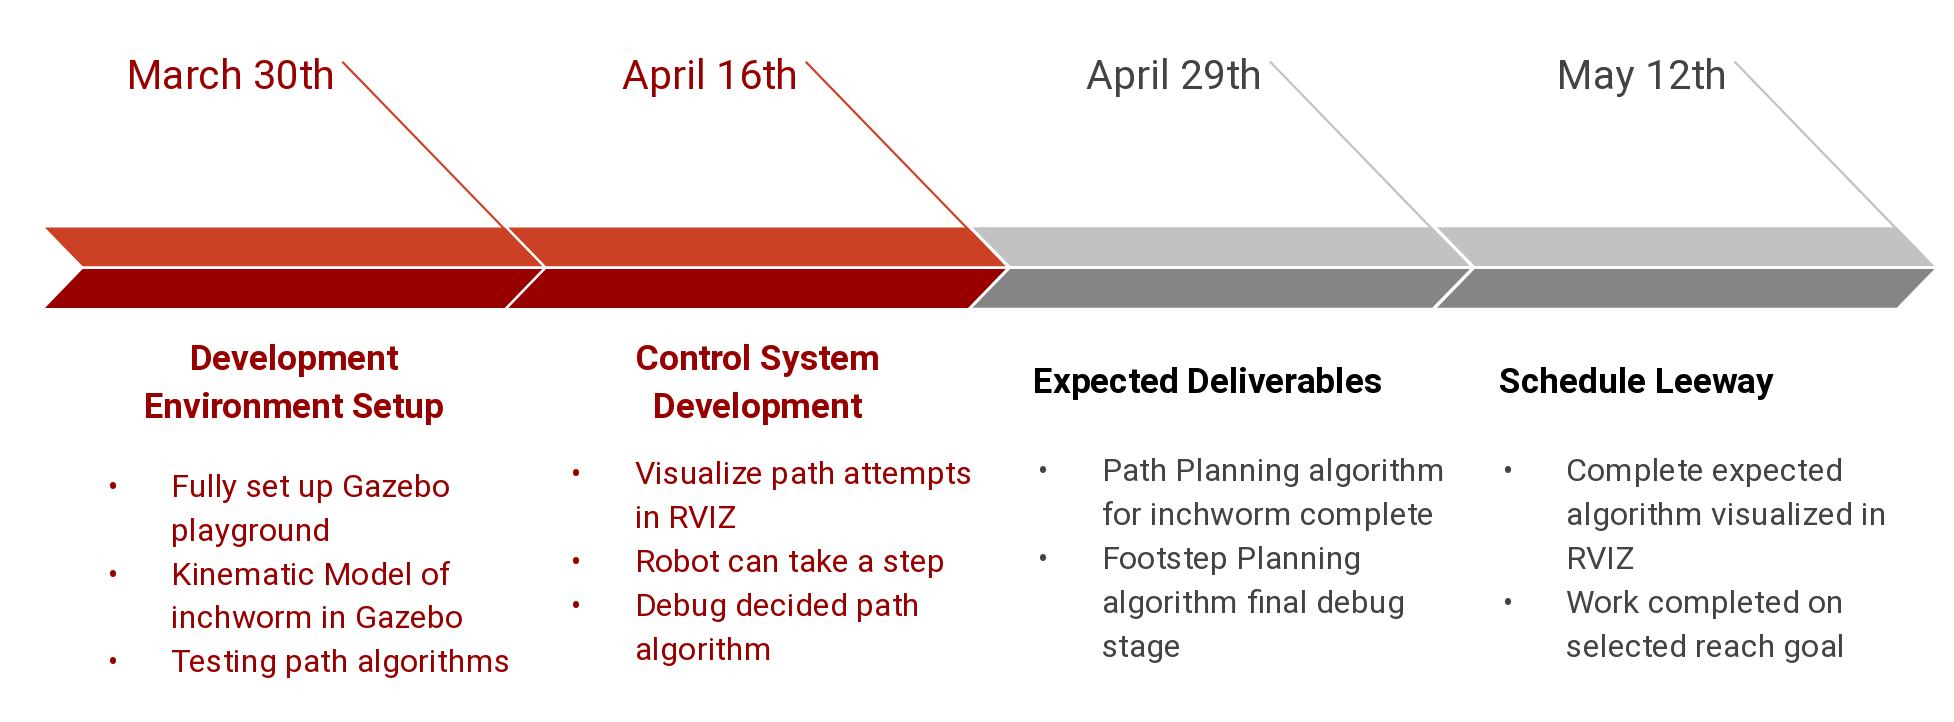
\includegraphics[width=\linewidth]{figures/Schedule.png}
    \caption{Proposed schedule for the project}
    \label{fig:Schedule}
\end{figure} 

    \printbibliography

\end{document}